\section{Experiments}
\label{sec:experiments}

In this section, we benchmark our continuous occlusion model for point-to-object association against the baseline method using detection bounding boxes and state-of-the-art methods for motion segmentation \cite{Rao_etal_2010,Brox_Malik_2010}. We then show how the proposed model may be applied for 3D localization in road scenes. For our experiments, we use the KITTI dataset~\cite{geiger2013vision}, which consists of video sequences of road scenes under a variety of driving conditions. 
%It also provides ground truth data for different tasks such as segmentation, detection, tracking and 3D localization.

%\paragraph{Dataset} We use KITTI dataset for our experiments.  \cite{geiger2013vision}. KITTI dataset is a labeled video sequence of road scenes under variety of driving conditions including highways and residential areas in Karlsruhe, Germany. It provides manually labelled ground truth data for localization of cars and also uses velodyne data provide metrically accurate estimates of cars location.


%%%%%%%%%%%%%%%%%%%%%%%%%%%%%%%%%%%%%%%%%%%%%%%%%%%%



\subsection{Association Experiments}
%\vspace{-0.2cm}
\paragraph{Setup}
We first perform the association experiment that compares the accuracy of point-to-object association using our proposed model against a heuristic baseline and state-of-the-art motion segmentation methods. The detection bounding box baseline method (BBox) is as described at the end of Section \ref{sec:association}. For motion segmentation, we use robust algebraic segmentation with hybrid perspective constraints (RAS)~\cite{Rao_etal_2010} and spectral clustering with point track spatial affinity (BM)~\cite{Brox_Malik_2010}.


\begin{figure*}[!!t]
\centering
%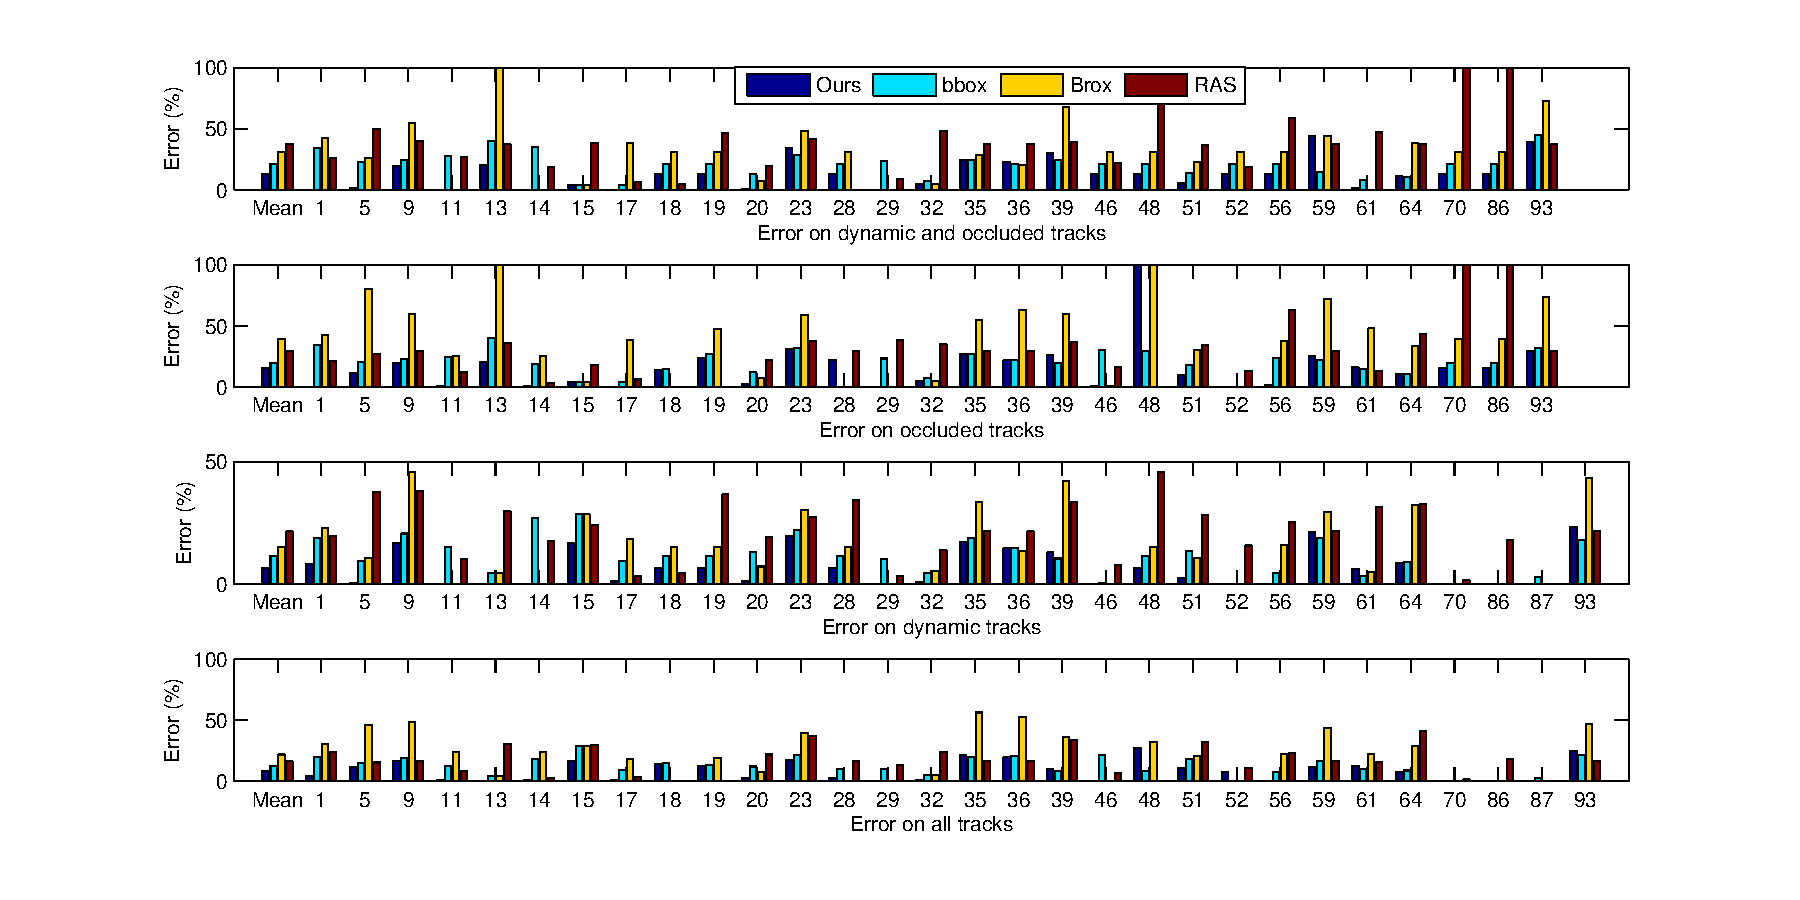
\includegraphics[trim=1.0in 0.4in 1.0in 0.2in, clip, width=\textwidth]{results/plotErrorBarEvalAssocCoeffAllSequence.pdf}
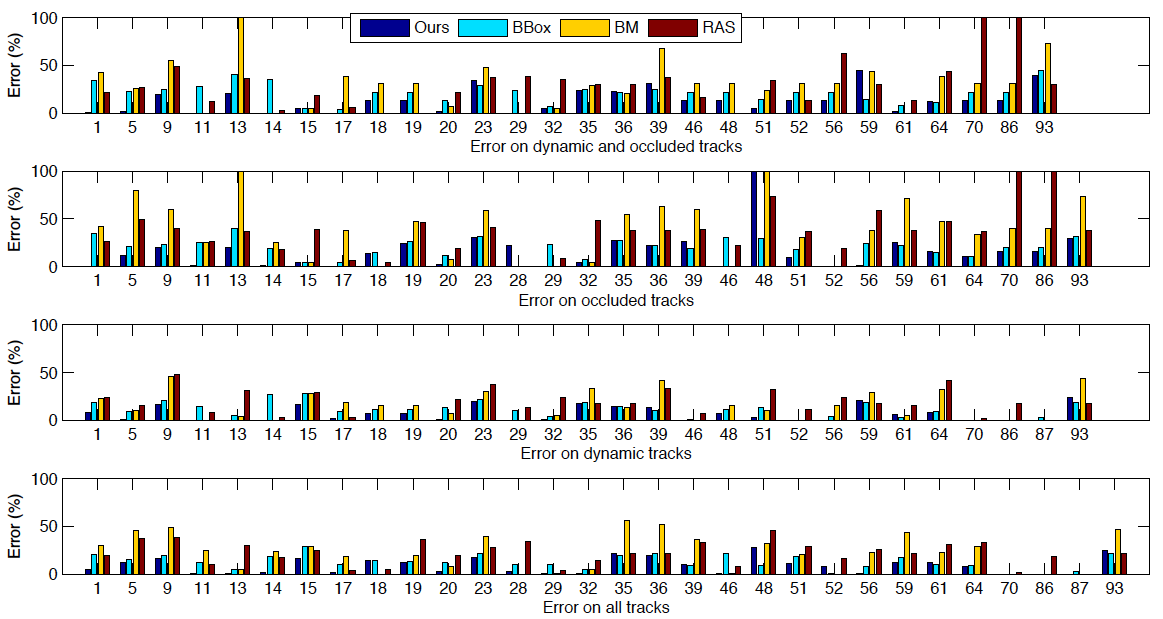
\includegraphics[width=0.95\textwidth]{graphics/figure5.png}
  \vspace{-0.3cm}
  \caption{\small Association errors on different sets of input point tracks. Numbers on y-axis represent data sequence numbers in KITTI dataset. Errors are in terms of average fractions of foreground points incorrectly associated to objects per sequence.}
  \vspace{-0.3cm}
  \label{fig:assoc-occ-results}
\end{figure*}

\begin{table}
\begin{tabular}{lrrrr}
  \toprule
  & Ours & BBox & BM & RAS\\
  \midrule
  Dyn. and occ. tracks        & \textbf{13.2} & 21.3 & 30.9 & 30.1 \\
  Occluded tracks             & \textbf{15.7} & 19.8 & 39.5 & 37.8 \\
  Dynamic tracks              & \textbf{06.6} & 11.4 & 15.3 & 17.7 \\
  All tracks                  & \textbf{08.6} & 12.6 & 21.9 & 21.5 \\
  \bottomrule
\end{tabular}
\caption{\small Mean association errors on different sets of input point tracks over all sequences of KITTI dataset. Errors are in terms of average fractions of foreground points incorrectly associated to objects per sequence.}
\label{tab:meanAssoc}
\end{table}


\newlength{\tblimgwidth}
\setlength{\tblimgwidth}{0.40\textwidth}
\begin{figure*}[!!t]
  \centering
  \begin{tabular}{ccc}
    & Associations & Error in association\\
    \rotatebox{90}{\hspace{2em} BBox} & 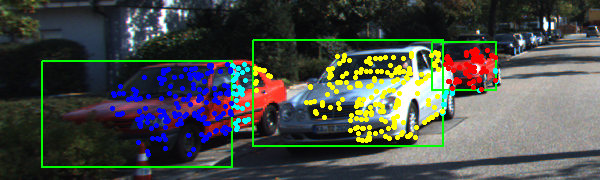
\includegraphics[width=\tblimgwidth]{results/0009_0000000060_point_assign_bbox2D_model-small.png} &%
    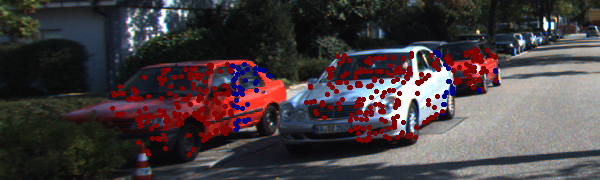
\includegraphics[width=\tblimgwidth]{results/0009_0000000060_point_assign_bbox2D_model_correct_incorrect-small.png}\\
    \rotatebox{90}{\hspace{2em} BM} & 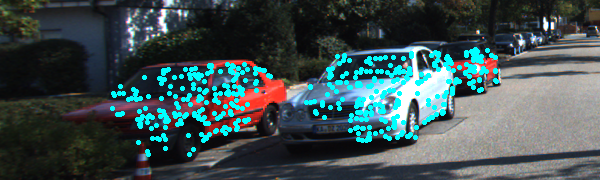
\includegraphics[width=\tblimgwidth]{results/0009_0000000060_point_assign_BroxAndMalik2010-small.png} &%
    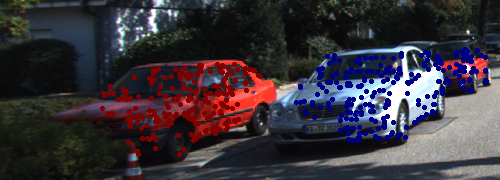
\includegraphics[width=\tblimgwidth]{results/0009_0000000060_point_assign_BroxAndMalik2010_correct_incorrect-small.png}\\
    \rotatebox{90}{\hspace{2em} RAS} & 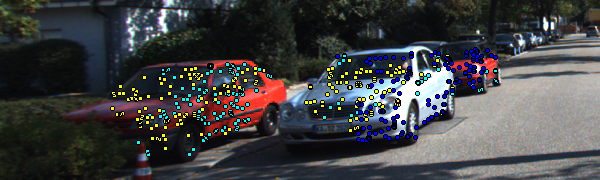
\includegraphics[width=\tblimgwidth]{results/0009_0000000060_point_assign_RAS-small.png} &%
    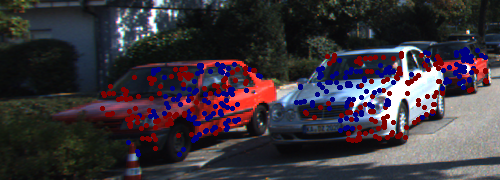
\includegraphics[width=\tblimgwidth]{results/0009_0000000060_point_assign_RAS_correct_incorrect-small.png}\\
    \rotatebox{90}{\hspace{2em} Ours} & 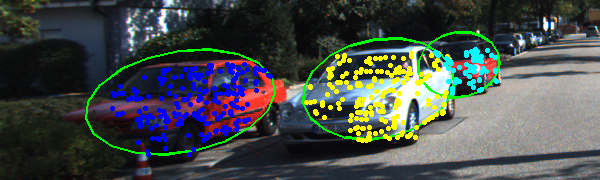
\includegraphics[width=\tblimgwidth]{results/0009_0000000060_point_assign_contPtTracks-small.png} &%
    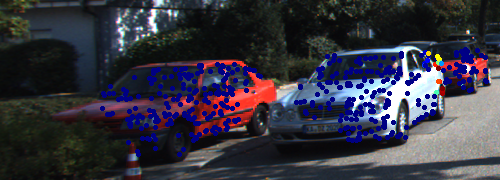
\includegraphics[width=\tblimgwidth]{results/0009_0000000060_point_assign_contPtTracks_correct_incorrect-small.png}\\
    \rotatebox{90}{\hspace{2em} BBox} & 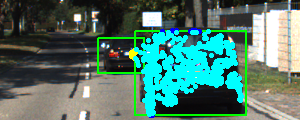
\includegraphics[width=\tblimgwidth]{results/0013_0000000060_point_assign_bbox2D_model-small.png} &%
    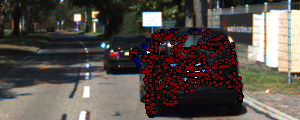
\includegraphics[width=\tblimgwidth]{results/0013_0000000060_point_assign_bbox2D_model_correct_incorrect-small.png}\\
    \rotatebox{90}{\hspace{2em} BM} & 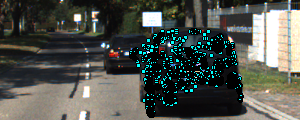
\includegraphics[width=\tblimgwidth]{results/0013_0000000060_point_assign_BroxAndMalik2010-small.png} &%
    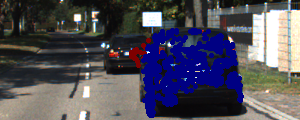
\includegraphics[width=\tblimgwidth]{results/0013_0000000060_point_assign_BroxAndMalik2010_correct_incorrect-small.png}\\
    \rotatebox{90}{\hspace{2em} RAS} & 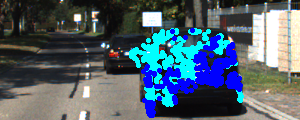
\includegraphics[width=\tblimgwidth]{results/0013_0000000060_point_assign_RAS-small.png} &%
    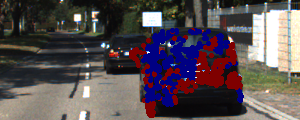
\includegraphics[width=\tblimgwidth]{results/0013_0000000060_point_assign_RAS_correct_incorrect-small.png}\\
    \rotatebox{90}{\hspace{2em} Ours} & 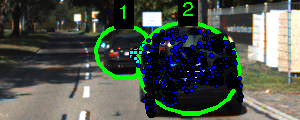
\includegraphics[width=\tblimgwidth]{results/0013_0000000060_point_assign_contPtTracks-small.png} &%
    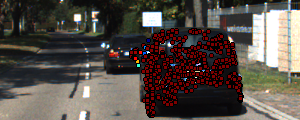
\includegraphics[width=\tblimgwidth]{results/0013_0000000060_point_assign_contPtTracks_correct_incorrect-small.png}
  \end{tabular}
  \vspace{-0.3cm}
  \caption{\small Qualitative results of the association experiment. The left column
  shows the point track assignments to appropriate objects. Each color represents
a different object to which point tracks can be associated to. Right column shows the
probabilistic error in association: low error points are in blue while high error points are in red.
Note that our method changes smoothly at the object boundaries with
intermediate probabilities, while the baseline method has merely 0-1 error.}
\label{fig:qualitative}
\vspace{-0.3cm}
\end{figure*}


%To verify the correctness of our association probability $\assocP$ we perform association error experiment that compare the accuracy of point track association with TPs with that of bounding box baseline method.

For each sequence of the KITTI dataset, the methods of \cite{Felzenszwalb_etal_2010} and \cite{Choi_Savarese_2010} are used for computing detection bounding boxes and object tracklets, respectively. We then apply \cite{Zach2007} to extract point tracks. Note that our method can handle occlusions in both static and dynamic scenes, but motion segmentation focuses on dynamic scenes. For a complete evaluation, we organize the point tracks into four sets: all point tracks, occluded point tracks, dynamic point tracks and dynamic as well as occluded point tracks. In addition to point tracks, the parameters of all objects (cars) estimated by the method of \cite{Song_Chandraker_2015} are provided to our method (for computing association probability) and the baseline BBox method (for depth ordering).


\vspace{-0.4cm}
\paragraph{Results}
Figure~\ref{fig:assoc-occ-results} shows the association errors -- the percentages of point tracks incorrectly assigned to objects -- for all methods on the four sets of input point tracks, for each sequence of the KITTI dataset. The mean results over all sequences are summarized in Table~\ref{tab:meanAssoc}. From Figure~\ref{fig:assoc-occ-results}, our method is usually the most accurate among all methods, leading to the best mean error on all sets of input point tracks in Table~\ref{tab:meanAssoc}, which is followed by the bounding box baseline method. This clearly shows the advantage of our continuous occlusion model over the simple baseline method for resolving occlusions. RAS and BM often have the highest errors in Figure~\ref{fig:assoc-occ-results}, thus, the highest mean errors on all sets of input point tracks in Table~\ref{tab:meanAssoc}. 

More importantly, both RAS and BM rely on motions of objects for clustering point tracks, therefore they cannot work well with static point tracks (for example, point tracks that belong to parked cars). This fact can be observed in Table~\ref{tab:meanAssoc}, where there are large differences in the mean errors of both methods on data containing static point tracks (rows 2 and 4) and data consisting of dynamic point tracks only (rows 1 and 3). In contrast, our method and the baseline method are relatively independent of object motions, resulting in smaller performance gaps. Further, our method also outperforms motion segmentation on dynamic objects (row 3), which shows the effect of detection bounding boxes and by a more significant margin when occlusions are present (row 1), which shows the effect of our occlusion modeling.

Qualitative comparisons of point track associations from various methods are shown in Figure \ref{fig:qualitative}. We note the low errors using our occlusion model and the smooth transition of assignment across object boundaries.



%  seqName   seqNum    Energy_description                                                    windows         t      yaw             dim        
%    City      1       contPtTracksNoOcc_ctBBoxNoOcc_size_posTmcmc_inference      9/18  5.811142 0.696358        1.961227        
%    City      1       contPtTracksNoOcc_contBBoxOcc_size_posTmcmc_inference      8/18  4.501543 0.786599        2.375481        
%    City      1       contPtTracks_ctBBoxNoOcc_size_posTmcmc_inference           8/18  3.932855 0.766397        2.222919        
%    City      1       contPtTracks_contBBoxOcc_size_posTmcmc_inference           8/18  4.928155 0.806356        2.287911        
% OccCity      1       contPtTracksNoOcc_ctBBoxNoOcc_size_posTmcmc_inference      9/18  3.953464 0.442196        1.720844        
% OccCity      1       contPtTracksNoOcc_contBBoxOcc_size_posTmcmc_inference      8/18  4.815849 0.463034        2.159956        
% OccCity      1       contPtTracks_ctBBoxNoOcc_size_posTmcmc_inference           8/18  4.058560 0.995495        1.593641        
% OccCity      1       contPtTracks_contBBoxOcc_size_posTmcmc_inference           8/18  3.241853 0.631901        2.167446        
% \begin{table}
%   \centering
%   \begin{tabular}{lrrr}
%     \toprule
%     Energy & t & yaw & dim \\
%     \midrule
%     $\EnergyTrackNoOcc + \EnergyBBoxNoOcc +\EnergySize+\EnergyDyn$
%     5.81 & 0.69 & 1.96 \\
%     $\EnergyTrackNoOcc + \EnergyBBox +\EnergySize+\EnergyDyn$
%     4.50 & 0.78 & 2.37 \\
%     $\EnergyTrack + \EnergyBBoxNoOcc +\EnergySize+\EnergyDyn$
%     3.93 & 0.76 & 2.22 \\
%     $\EnergyTrack + \EnergyBBox +\EnergySize+\EnergyDyn$
%     4.92 & 0.80 & 2.28 \\
%     \bottomrule
%   \end{tabular}
%   \caption{Localization experiment results with different combination of energies. We report error in three metrics translation error (t) in meters per car, yaw error (yaw) in radians per car and dimension error is again meters per car.}
%   \label{tab:localizationExperimentNoOcc}
% \end{table}

%% \begin{table}
%% \small
%%   \begin{tabular}{lrrr}
%%     \toprule
%%     Energy & t & yaw & dim \\
%%     \midrule
%%     $\EnergyTrackNoOcc + \EnergyBBoxNoOcc +\EnergySize+\EnergyDyn$ 
%%     & 3.95 & 0.44  & 1.72\\        
%%     $\EnergyTrackNoOcc + \EnergyBBox +\EnergySize+\EnergyDyn$        
%%     & 4.81 & 0.46  & 2.16\\        
%%     $\EnergyTrack + \EnergyBBoxNoOcc +\EnergySize+\EnergyDyn$      
%%     & 4.05 & 0.99  & 1.59\\        
%%     $\EnergyTrack + \EnergyBBox +\EnergySize+\EnergyDyn$             
%%     & 3.24 & 0.63  & 2.16\\
%%     \bottomrule
%%   \end{tabular}
%%   \caption{\small Localization experiment results with different combination of energies. We report error in three metrics translation error (t) in meters per car, yaw error (yaw) in radians per car and dimension error is again meters per car. The results provided here are only on occluded tracks.}
%%   \label{tab:localizationExperiment}
%% \end{table}


\begin{table}
  \begin{tabular}{lrr}
    \toprule
    Energy & t & dim \\
    \midrule
    $\EnergyTrackNoOcc + \EnergyBBoxNoOcc +\EnergySize+\EnergyDyn$ 
    & 3.95  & 1.72\\        
    $\EnergyTrackNoOcc + \EnergyBBox +\EnergySize+\EnergyDyn$        
    & 4.81  & 2.16\\        
    $\EnergyTrack + \EnergyBBoxNoOcc +\EnergySize+\EnergyDyn$      
    & 4.05  & {\bf 1.59}\\        
    $\EnergyTrack + \EnergyBBox +\EnergySize+\EnergyDyn$             
    & {\bf 3.24}  & 2.16\\
    \bottomrule
  \end{tabular}
  \caption{\small Localization experiment results with different combinations of energies. We report translation error (t) and dimension error (dim) in meters per car. Yaw angles for static objects are not optimized by our model. These experiments use the set of occluded tracks to demonstrate the effect of our modeling.}
  \label{tab:localizationExperiment}
\end{table}


\subsection{Localization Experiments}
We report errors in translation and dimension estimates, measured in meters per car, in Table~\ref{tab:localizationExperiment}. Average depth of cars in the dataset is approximately $20$ meters. We compare four combinations of energies.  The energy $\EnergyTrackNoOcc$ represents the point tracks energy without accounting for occlusion, that is, we model $\EnergyTrack$ in the absence of $a^{ij} (\lambda)$. Similarly, $\EnergyBBoxNoOcc$ is the energy without the modification of $\Lambda_k$ that accounts for occlusion. We observe that the use of the continuous occlusion model improves the localization accuracy in terms of the translation error, which is the most significant metric affected by all cues. Occlusion modeling for detection increases dimension error since we explicitly allow greater uncertainty in occluded edges of the bounding box. Note that none of our energies optimize yaw angles for static objects, which can be handled in practice through either the detector orientation or external information such as lane geometry.

%of all three metrics: translation, yaw and dimension error.


%We report error in three metrics translation error (t) in meters per car, yaw error (yaw) in radians per car and dimension error is again meters per car. The results are shown in Table~\ref{tab:localizationExperiment}.  We compare four combinations of energies as shown in the table.  The energy $\EnergyTrackNoOcc$ represents the point tracks energy modeled with accounting for occlusion, i.e., we remove the term $\Ptransmission$ and model $\EnergyTrack$ in the absence of $\Ptransmission$. Similarly, $\EnergyBBoxNoOcc$ is the energy without the modification of $\Sigma^{(d)}_j$ that accounts for occlusion.  The results show that use of continuous occlusion model improves the localization accuracy in terms of all three metrics: translation, yaw and dimension error.

